\chapter{Experimental results obtained}
%\chapter*{Concluzii}
\section{Data processing}
The process of defining and training both the classification model and the detection model started with gathering the data and learning how to work with dcm files because this was the first time I had an encounter with them. I quickly discovered that reading the images from the dcm files took a lot of time, which meant that training the models would also take a lot of time. These files contained the pixel data of about 50 slices, some had more and some had less, each representing images of width 2457 and height 1890, or 1996. I searched for ways to reduce the time for reading the files, at first by saving the slices as numpy arrays in file format, but that proved to not be ideal because it occupied a lot of disk storage. The dcm files themselves were not light either, totaling 120 GB of memory on my laptop, but the numpy arrays would have been impossible to store. Then, I arrived at the solution that, in time, proved to be the best: to save each individual slice as a png file. This meant that the time for reading the images was much faster, reading from dcm compared to png, and also that disk space was better utilized.\\
In ~\cite{carte8} it is said that the input images for the object detection model should have a size divisible by 128, which I was not aware of when training the classification model, for which the images were not resized at all. I was training images of size 2457,1890 on the GoogleNet model, but only taking a maximum of 5 slices from each image. After processing the dcm files, I found out that the lowest number of slices for an image in my entire subsection of the database was 22 therefore, for the purpose of properly balancing the database, I took into consideration only 22 slices of each image. For the images that had cancer, the ones that I had a file of bounding boxes on, I took the slice that had the tumor, 10 slices before that, and 11 after.\\
\section{Classification experiments}
I performed many experiments on the GoogleNet model for classification, and so I was able to understand how to work with 3D images. I first thought I had to stack them, so I sent the 5 slices that I selected from each image as 5 channels for the same input. That meant modifying the first convolutional layer of the GoogleNet architecture, which accepted inputs of 3xWxH.\\
The first experiment was made with a learning rate of 0.001, no learning rate decay, the optimizer was SGD, and the loss for every experiment, including this one, was cross-entropy. However, for the first few runs, I considered the problem of classification as a 4 label distinction, for which I attributed a different weight to the 4 labels: 1 for both normal and actionable, and 4 for benign and malign. The batch size was 10, and the images were not resized, so I was training images of width 2457 and height 1890. The batches were also not properly distributed, meaning that one single batch could have images of only one type. Each input consisted of 5 slices stacked on top of each other, representing 5 channels.\\
In order to track and compare each experiment, I used Weights \& Biases, also known as wanb, and logged the loss for each step, meaning that after each batch, the loss was calculated and added to the overall graph. Therefore, the image below shows the loss graph for the experiment described above.\\
\begin{figure}[ht!]
    \centering
    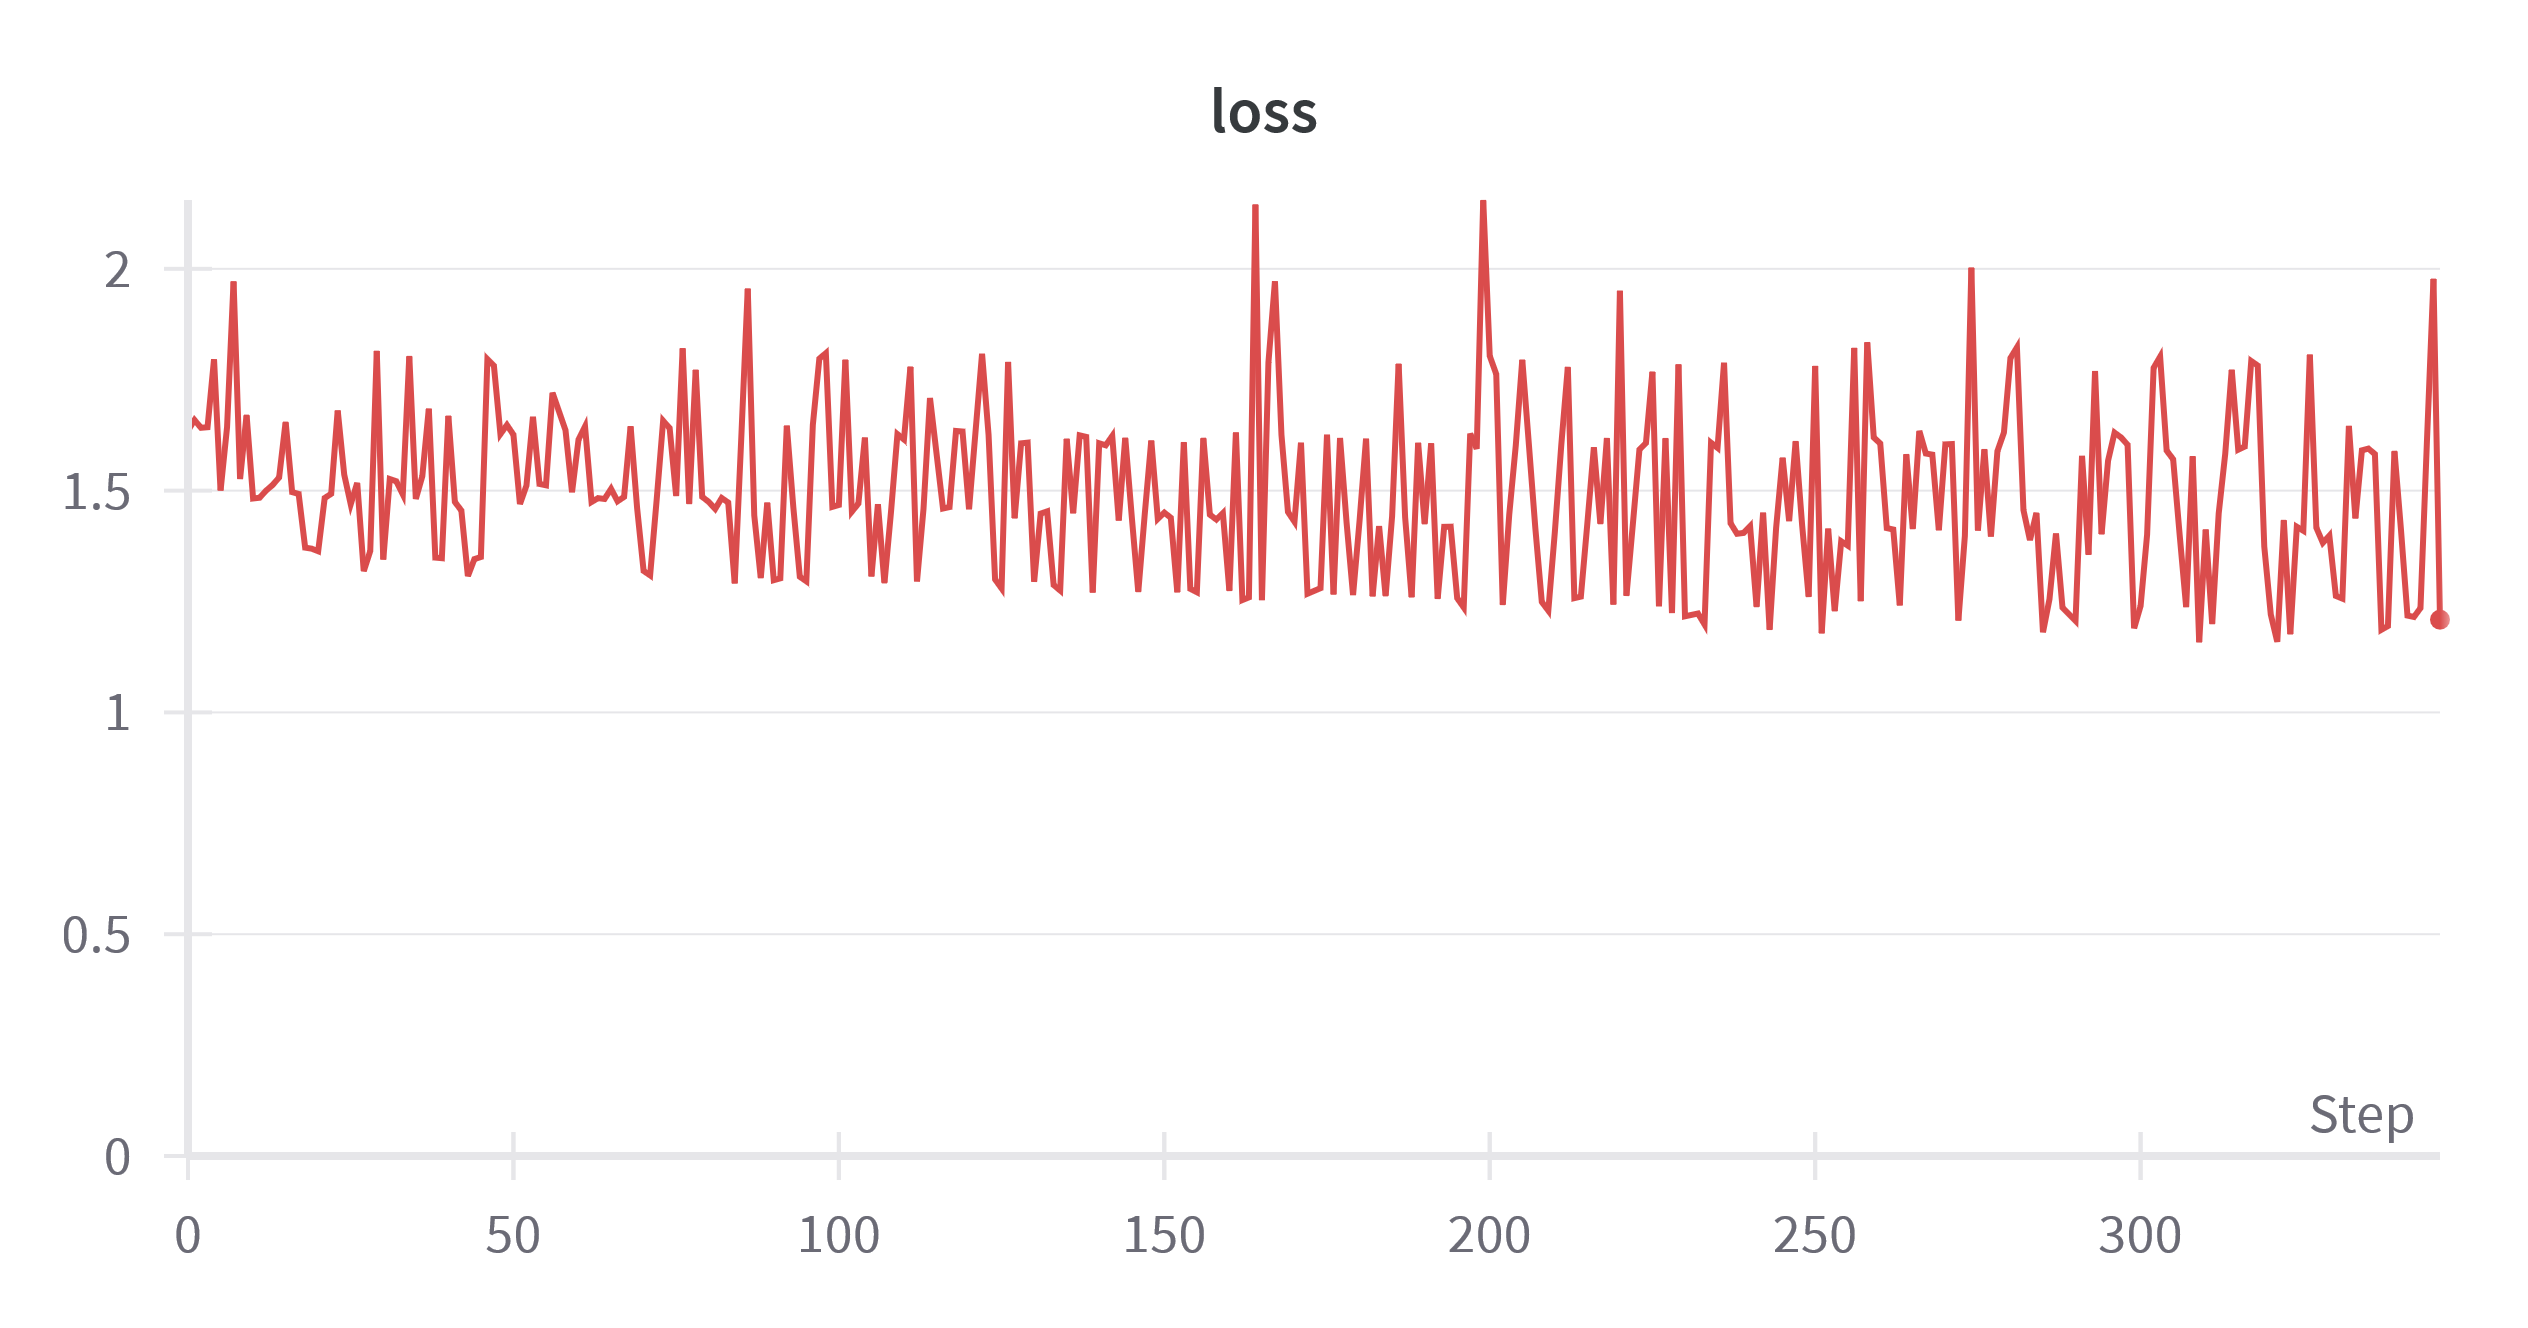
\includegraphics[width=1\textwidth]{figures/Figure8.png}
    \caption{Loss Graph}
    \label{fig:fig8}
\end{figure}
Evidently, the loss is not ideal. It does not appear to reduce its value after each step. This image consists of the loss of the model calculated for 6 epochs, and the predictions made on the test data was not ideal either, because it seemed to only predict normal or actionable types, disregarding the latter ones entirely. This is how the confusion matrix looked after the first epochs, and after the sixth one.\\
\begin{figure}[ht!]
    \subfigure[]{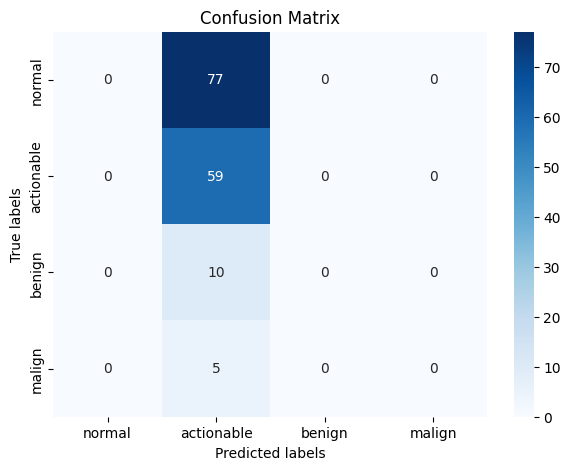
\includegraphics[width=0.45\linewidth]{figures/Figure9.png}}
    \subfigure[]{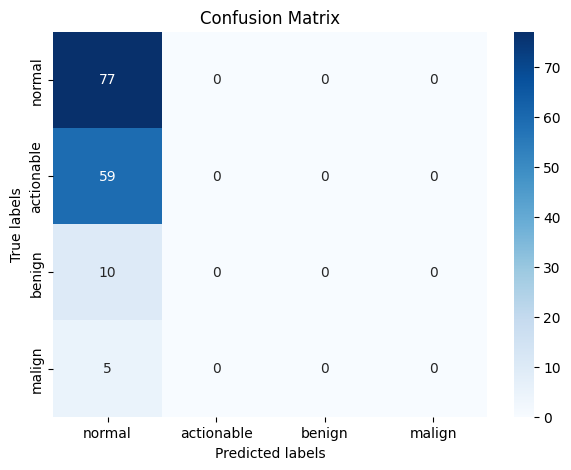
\includegraphics[width=0.45\linewidth]{figures/Figure10.png}}
    \caption{(a) After epoch 1 (b) After epoch 6}
    \label{fig:fig9}
\end{figure}
The second experiment proved to be a little more fruitful. I changed the learning rate to 0.0001, the optimizer to Adam and employed learning rate decay, more exactly a step learning rate decay with a step size of 4 and a gamma of 0.1. The batch size was changed to 8 and I utilized a batch sampler class to correctly distribute the different input types into the batches in order to have a better proportion of classes. I was also under the impression that the GoogleNet architecture was maybe too deep to predict the images, so I experimented with the two auxiliary modules that GoogleNet provides. For this experiment, I trained the model using the first auxiliary while also modifying the forward-pass function to only include two inception layers.\\
Additionally, I changed the weights for the benign and malign classes in the loss function, substituting 4 for 6 for both of them. Image \ref{fig:fig10} show how the loss graph looked after training eight epochs and another 21 batches in the ninth epoch.\\
\begin{figure}[ht!]
    \centering
    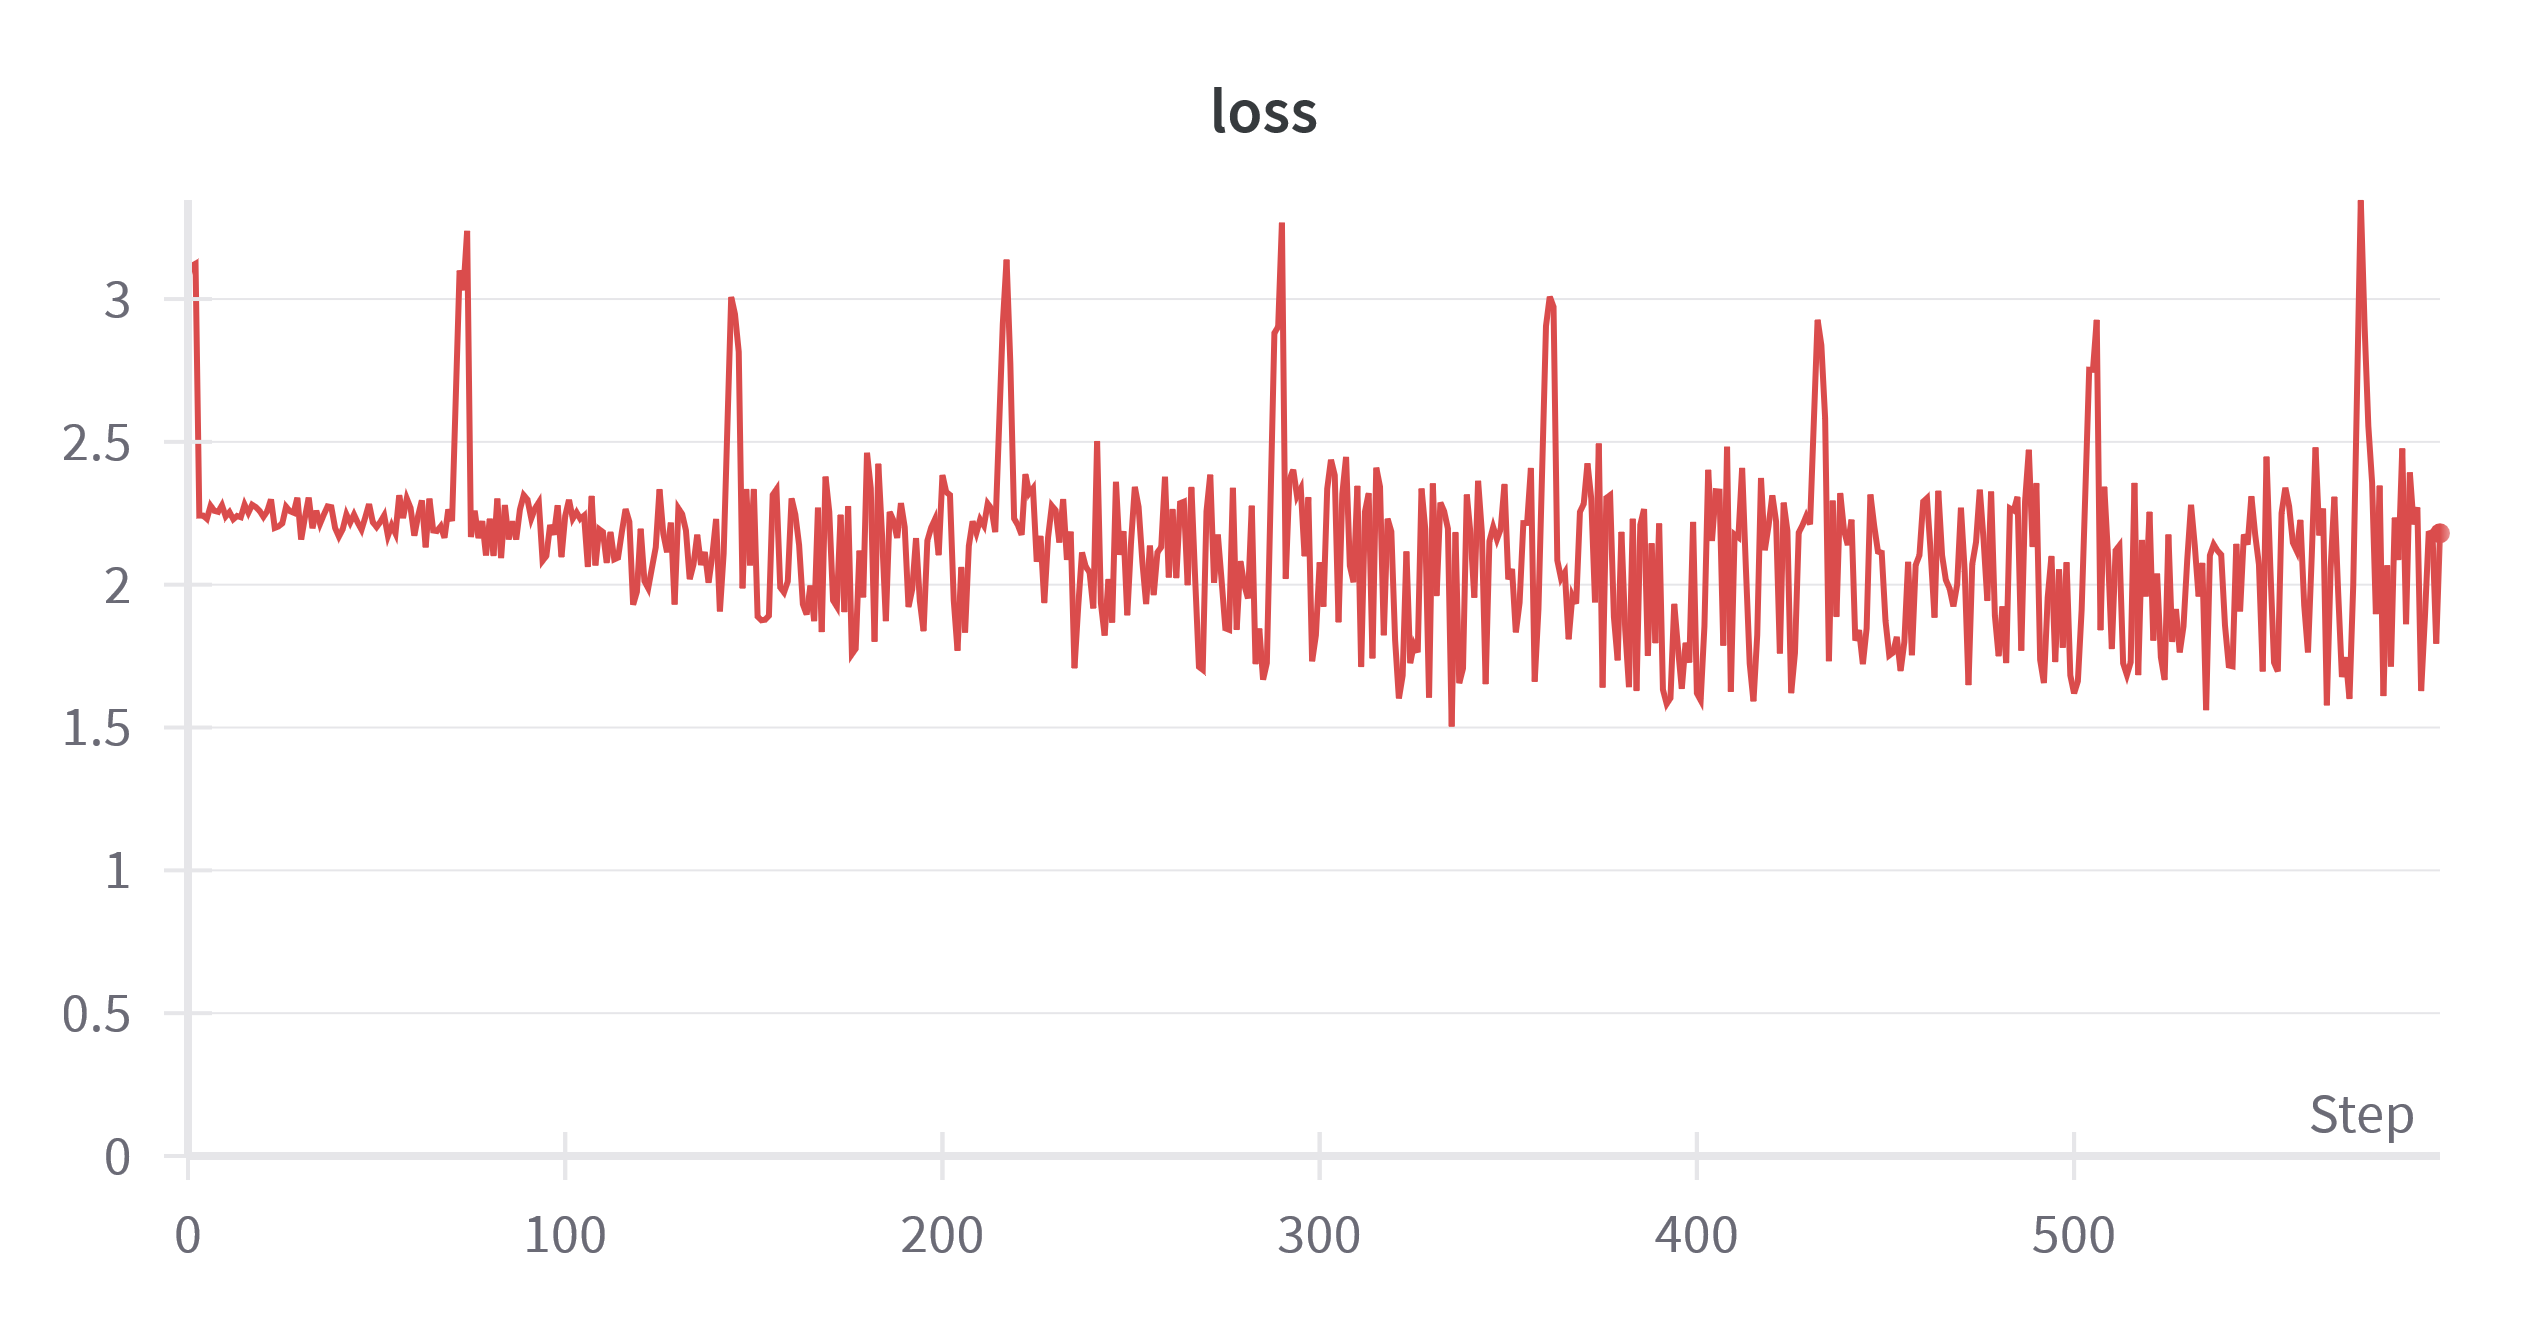
\includegraphics[width=1\textwidth]{figures/Figure11.png}
    \caption{Loss graph}
    \label{fig:fig10}
\end{figure}
This time around, the model started to also predict images of class malign, but only after the first epoch. Curiously, it did not predict any images to be of type benign, even after eight epochs. Image \ref{fig:fig11} show how the predictions looked after the first and eighth epochs.\\
\begin{figure}[ht!]
    \subfigure[]{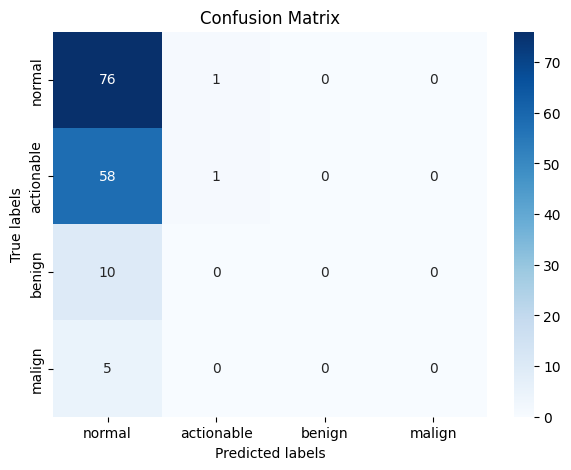
\includegraphics[width=0.45\linewidth]{figures/Figure12.png}}
    \subfigure[]{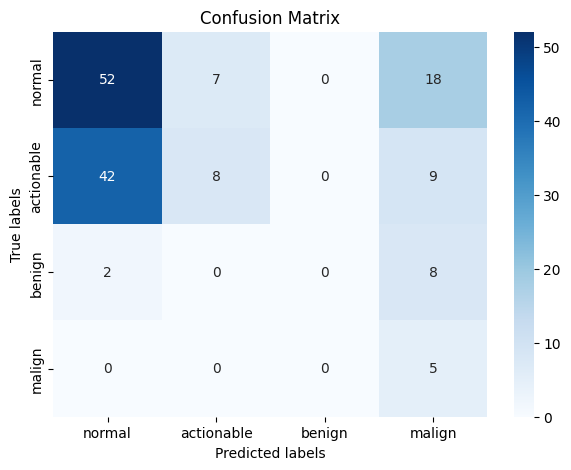
\includegraphics[width=0.45\linewidth]{figures/Figure13.png}}
    \label{fig:fig11}
    \caption{(a) After epoch 1 (b) After epoch 8}
\end{figure}
The only difference between this second experiment and the third was that the learning rate decay was changed from step to exponential with a gamma of 0.8. Below is shown on the same graph the difference in loss between these two latter experiments.\\
\begin{figure}[ht!]
    \centering
    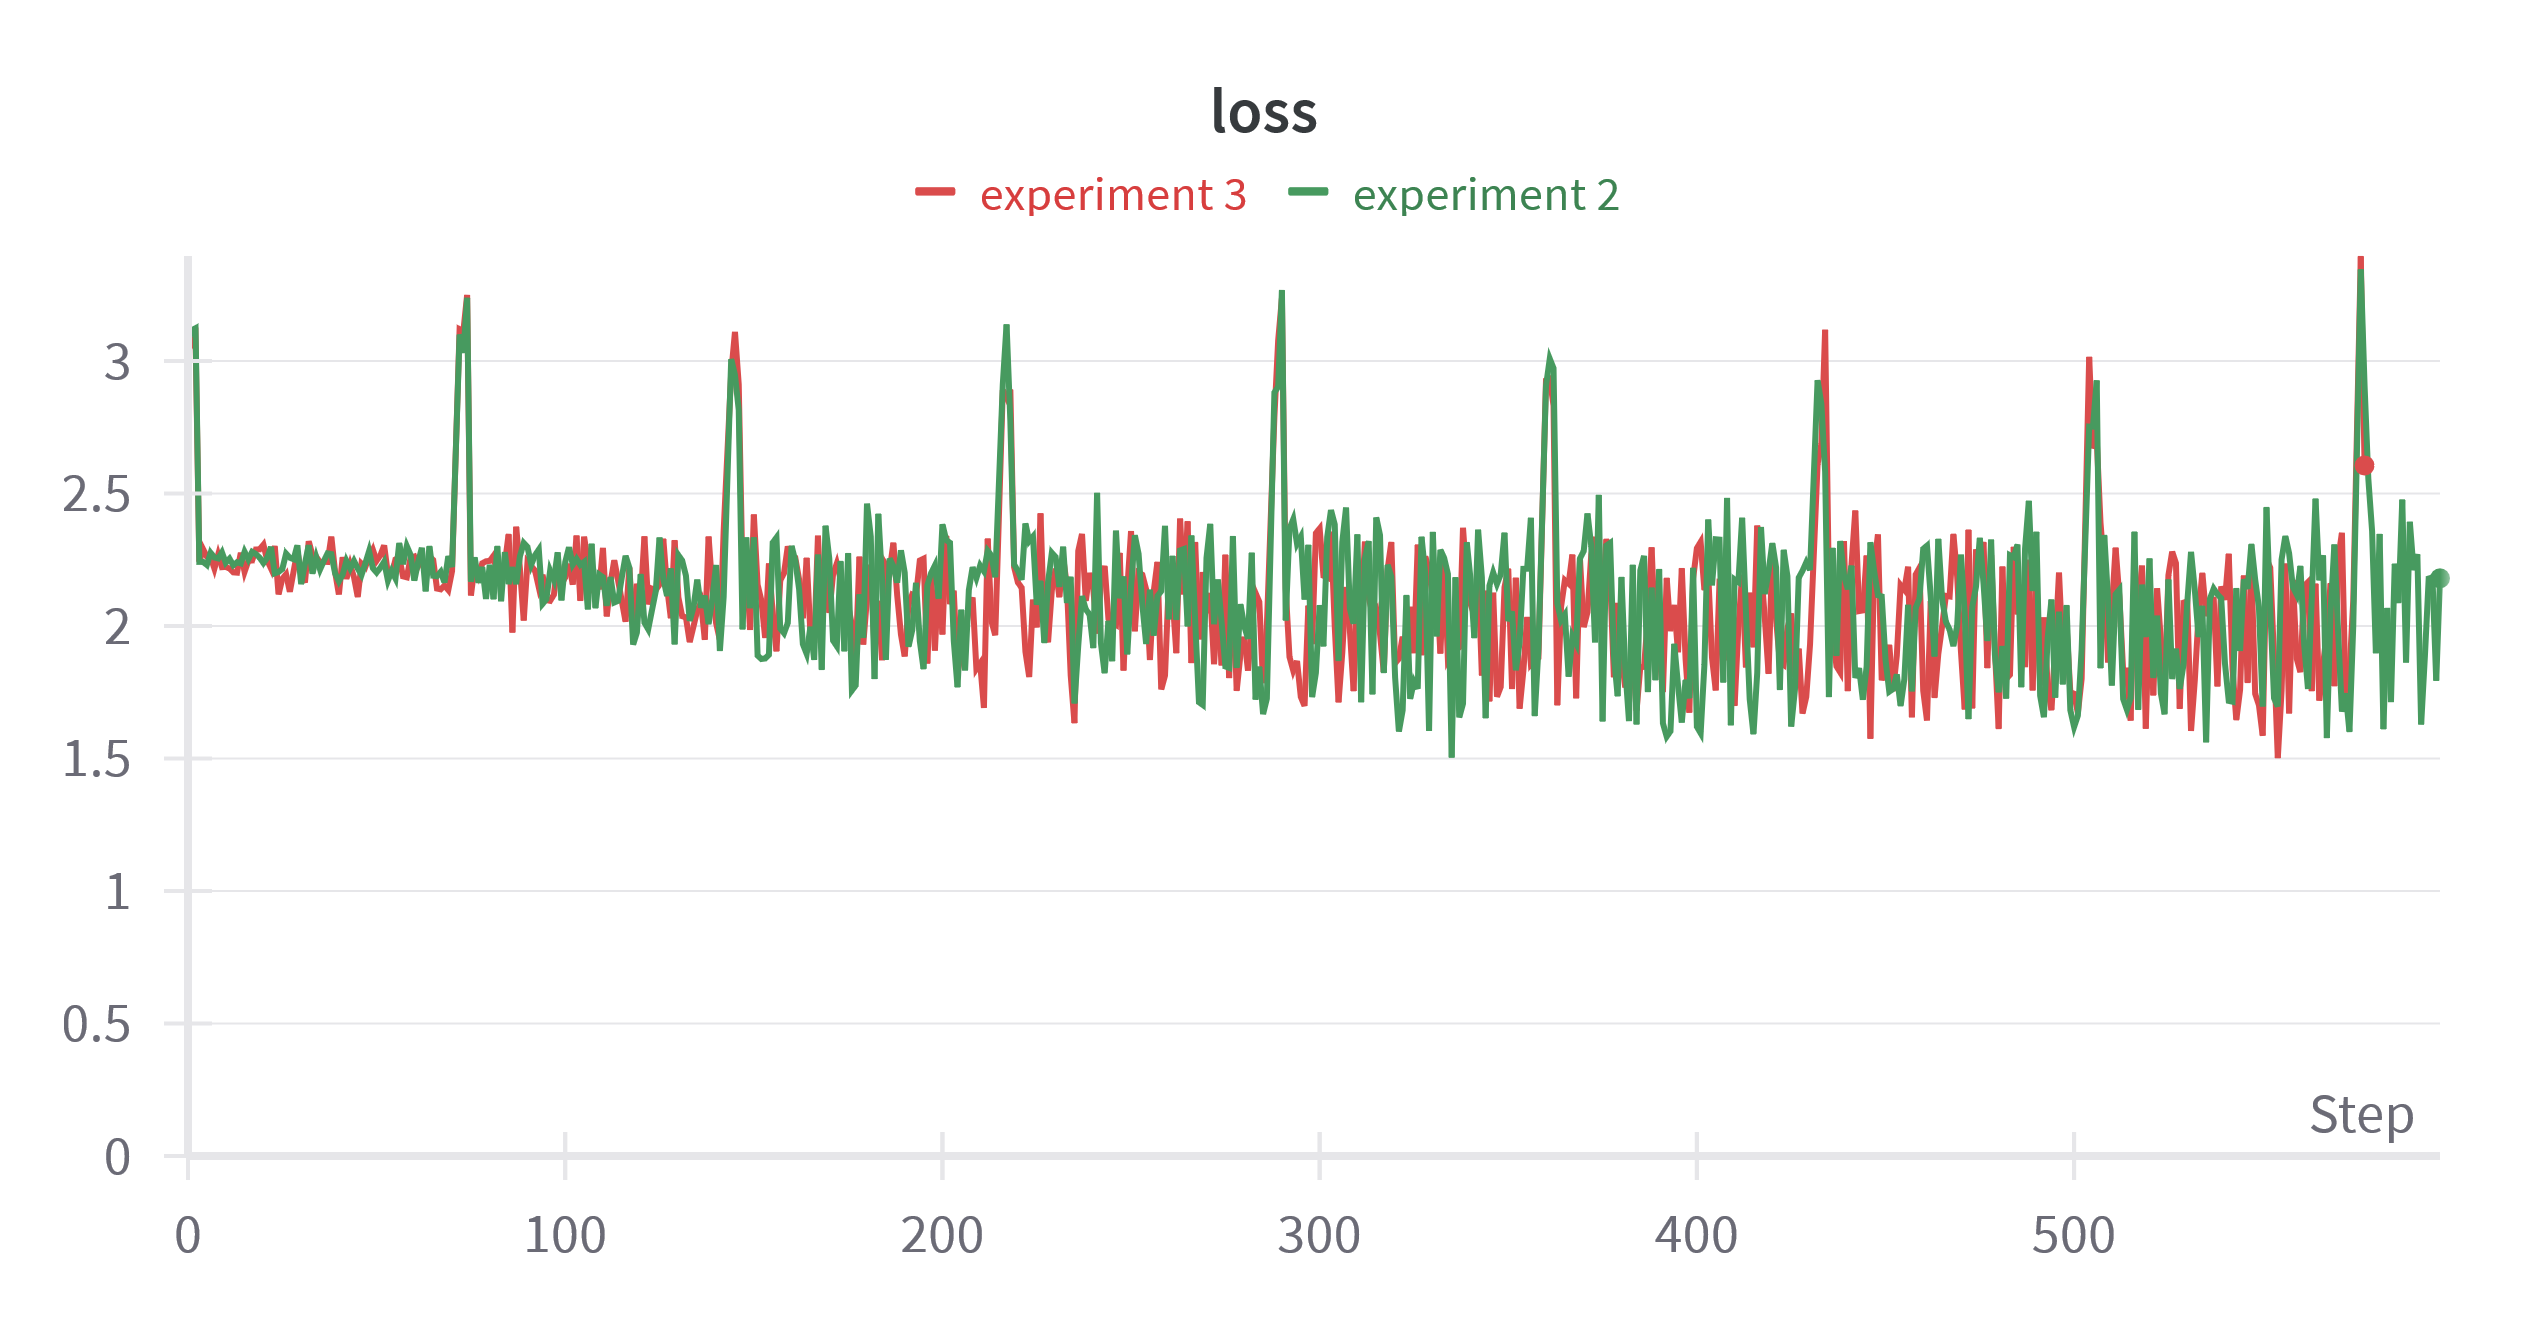
\includegraphics[width=1\textwidth]{figures/Figure14.png}
    \caption{Loss graph}
    \label{fig:fig13}
\end{figure}
The predictions for the third experiment were very similar to the ones from the second experiment, meaning the model would predict only three classes out of all four of them.\\
The spikes in image \ref{fig:fig10} represent the batches that had more input of classes benign and malign because the number of classes did not allow for equally proportionate batches of eight. I thought that the randomness in which these batches appeared could negatively impact the overall accuracy of the model, so in further experiments, I changed this way of thinking and made these batches appear first. This is how the experiment turned out, so not much was changed, and the predictions overall on the test data were not different.\\
\begin{figure}[ht!]
    \centering
    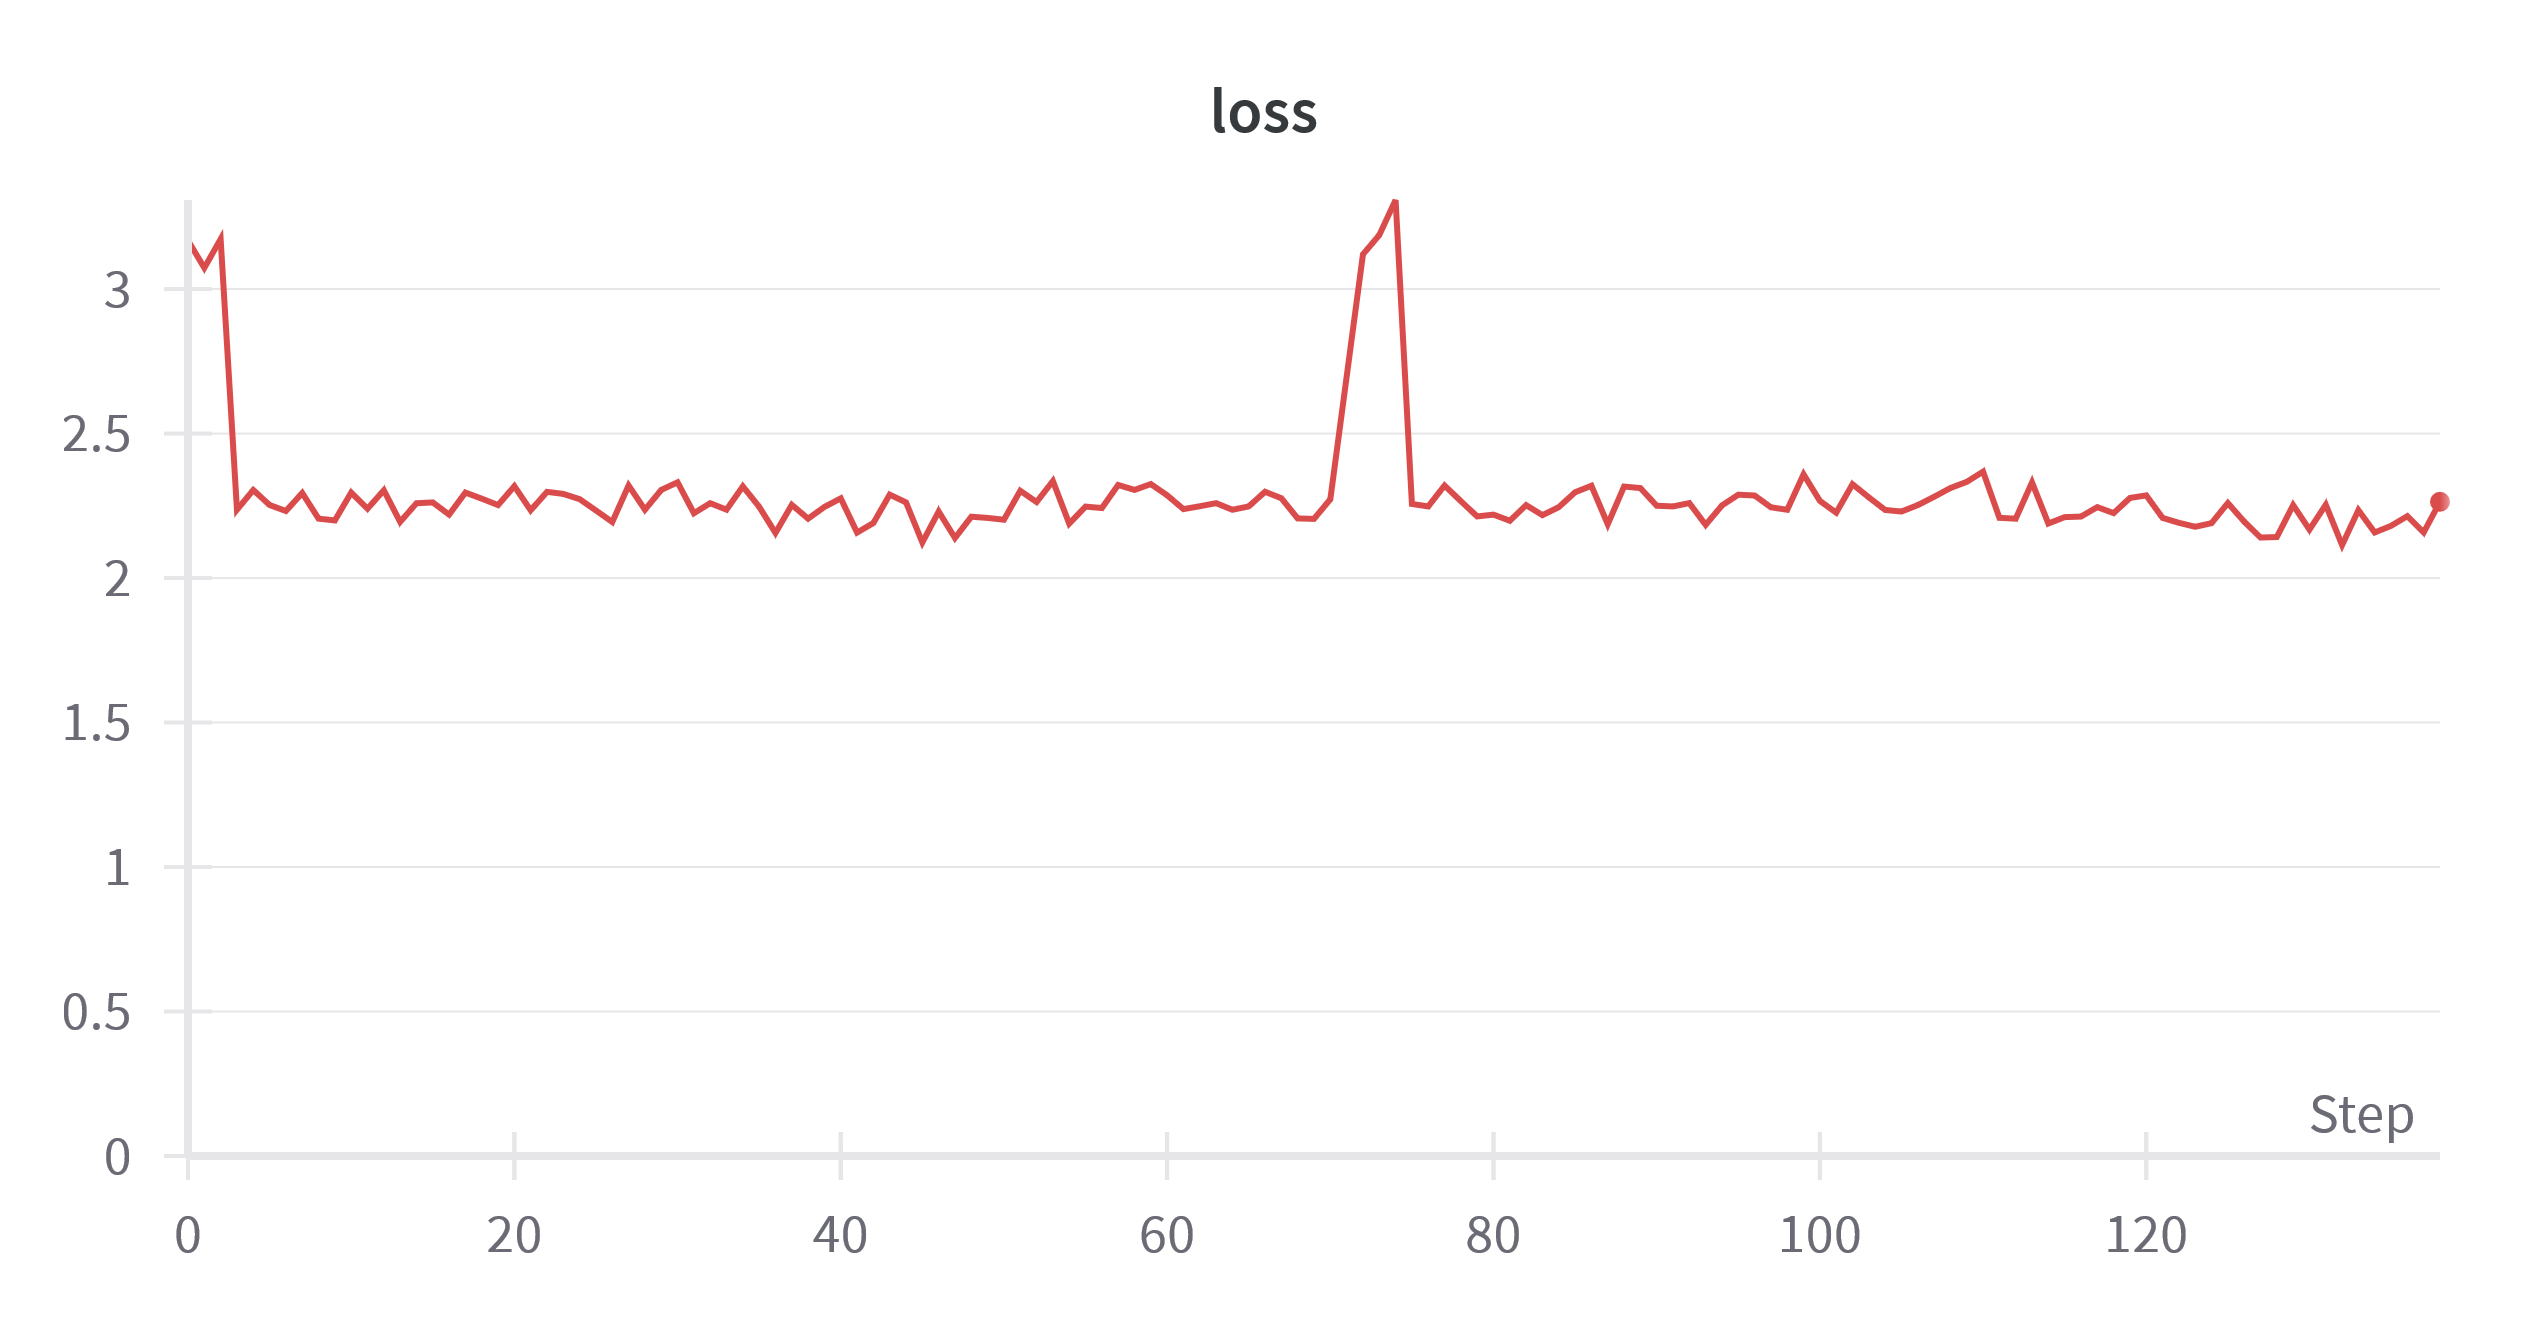
\includegraphics[width=1\textwidth]{figures/Figure15.png}
    \caption{Loss graph}
    \label{fig:fig14}
\end{figure}
For the next experiment, I stopped considering this a problem of 4-label detection but rather a 2-label detection. Therefore, I grouped the actionable, benign and malign types into one and trained the model using this group and the normal ones. I kept everything else in terms of configuration from the third to the fourth experiment, except for batch size, which I changed to 64. Image \ref{fig:fig16} shows how the loss looked after training three epochs, and image \ref{fig:fig7} shows how the confusion matrix looked after those three epochs.\\
\begin{figure}[ht!]
    \centering
    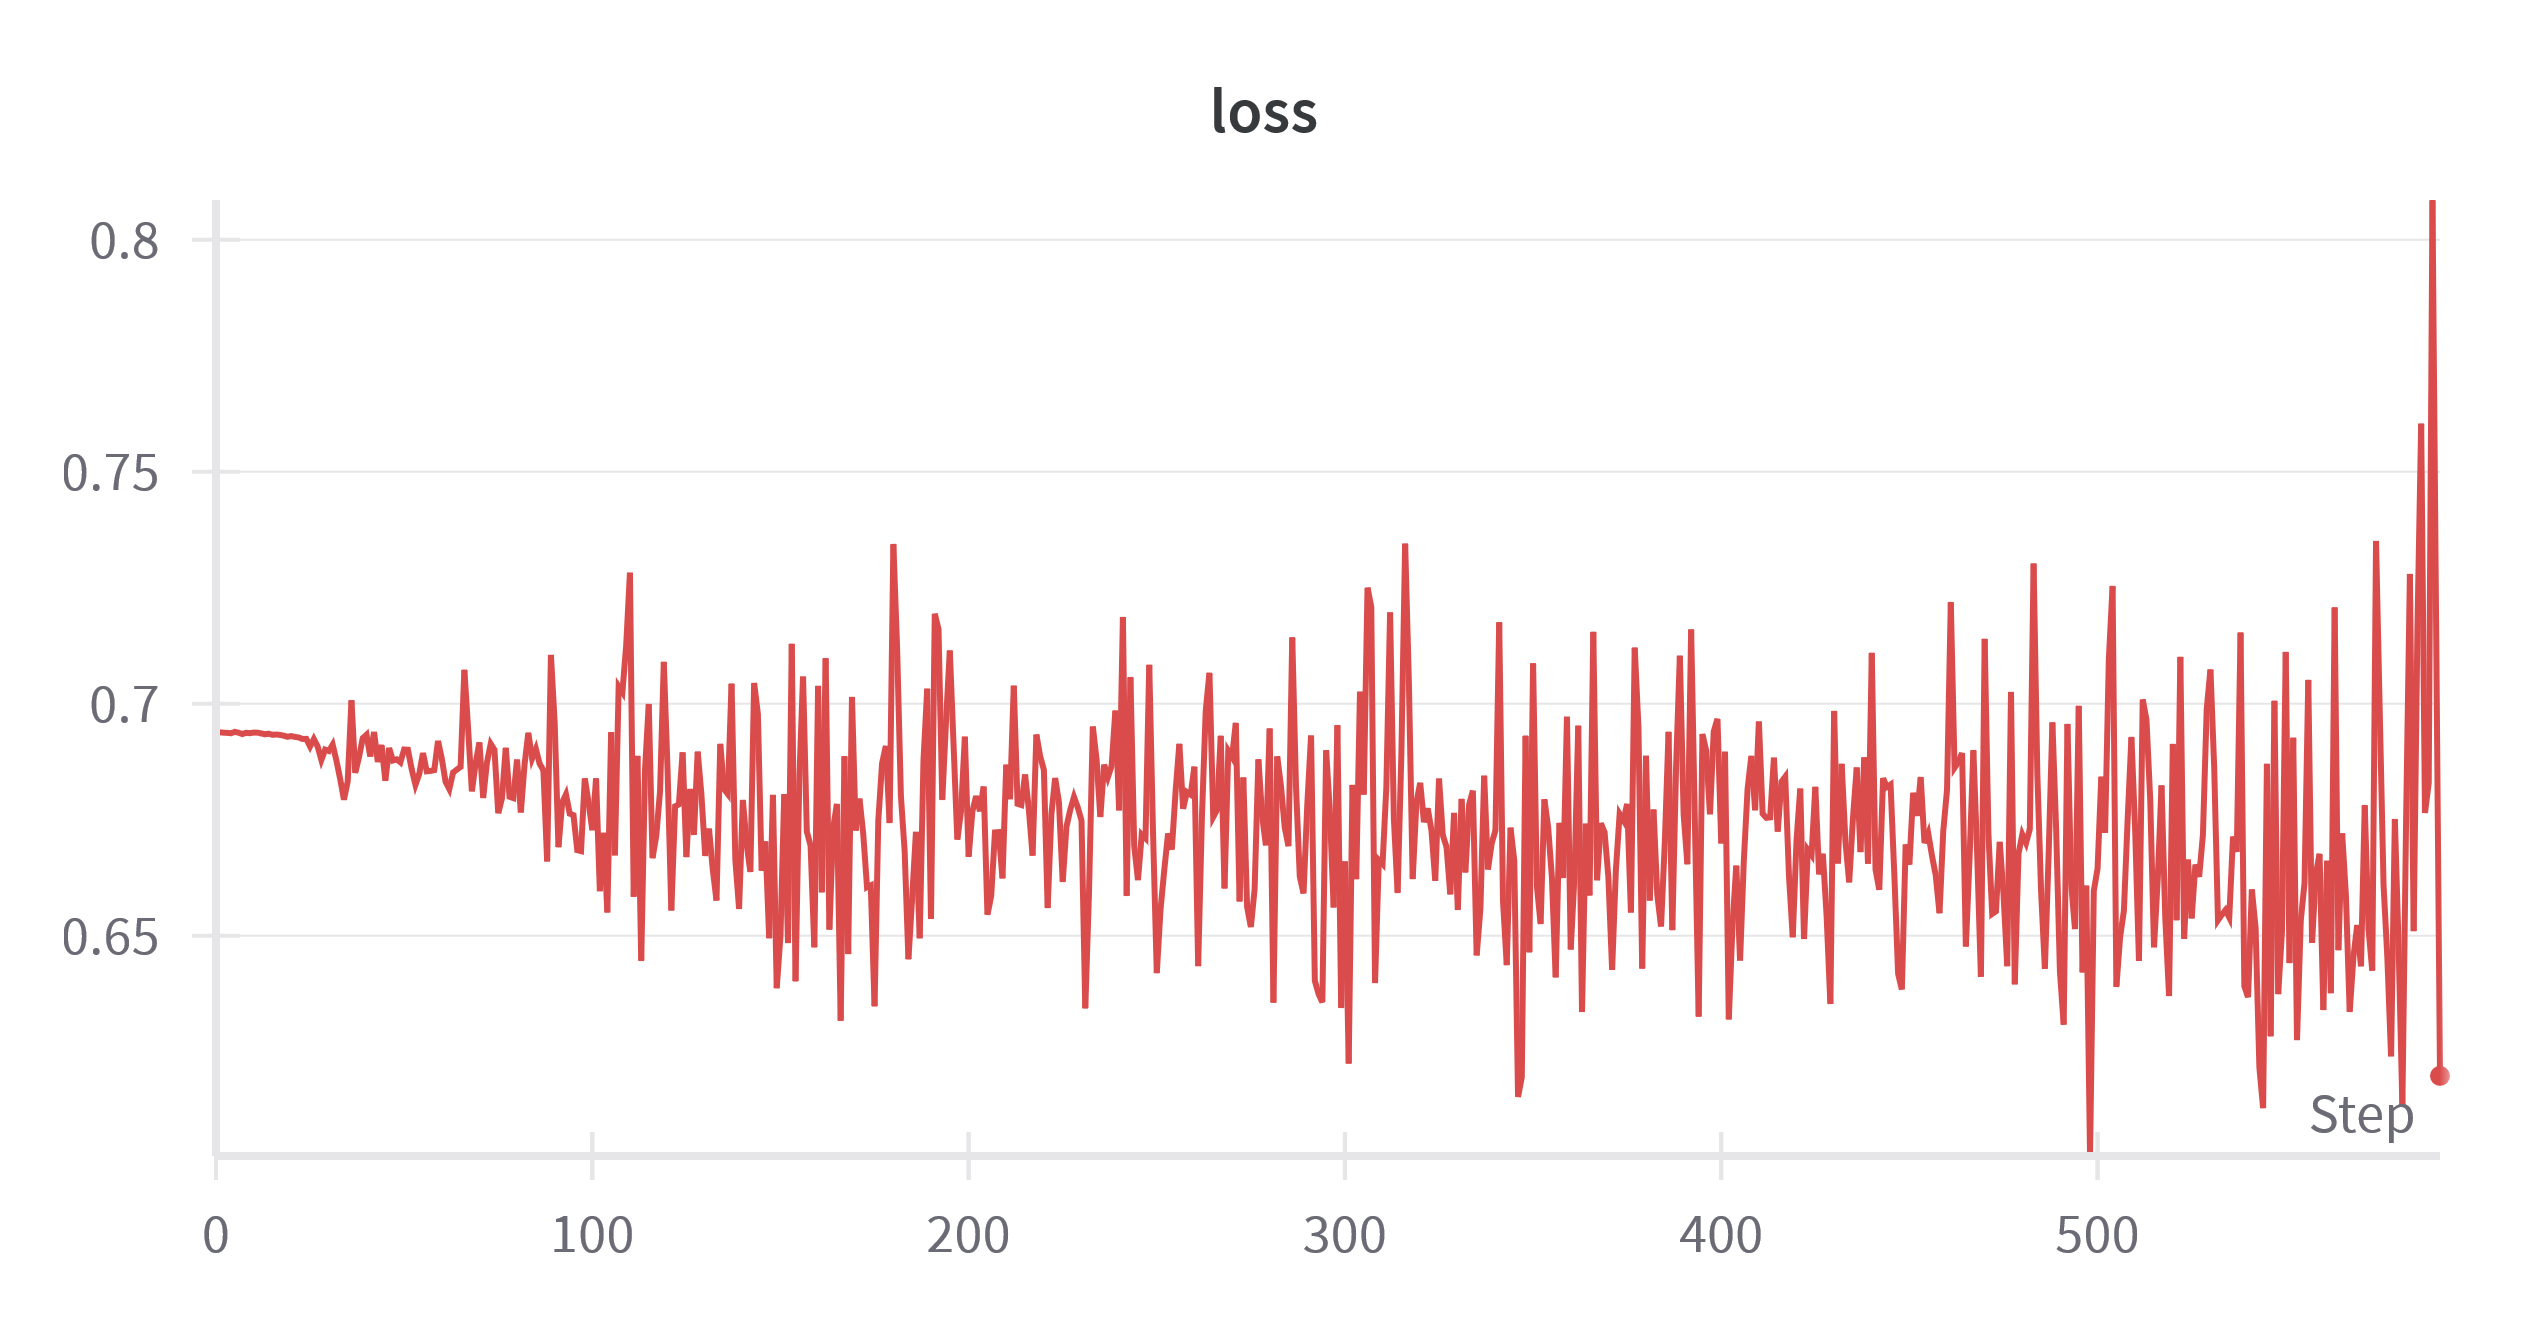
\includegraphics[width=1\linewidth]{figures/Figure17.png}
    \caption{Loss graph}
    \label{fig:fig16}
\end{figure}
\begin{figure}[ht!]
    \centering
    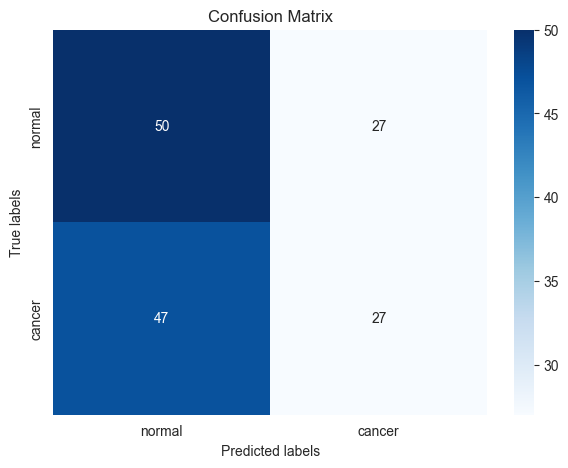
\includegraphics[width=0.5\linewidth]{figures/Figure18.png}
    \caption{After 3 epochs}
    \label{fig:fig17}
\end{figure}
I resized the images to be 300x300 and instead of adding the slices as channels of the same image, I added the slices as individual inputs. In doing so, I transformed a 568-length dataset into a 2,840-length one, and used a batch size of 64.\\
Upon figuring out the number of learnable parameters, which was around 3 milions, I wanted to increase the length of the dataset even more. With this purpose in mind I considered 22 slices of each input, and adding each of them individually resulted in a 12,496-length dataset.\\
Additionaly, I wanted to compare the loss of the two auxiliary models that GoogLeNet has to offer with the main output that it returns. In doing so, i returned to the initial implementation for the forward-pass method. However, I made a mistake in that I forgot that the original implementation doesn't include either activation function on the last layer, instead adding one only for the main output, not for the two auxiliary modules. Curiously, these two modules proved to obtain the lowest loss of all the experiments I performed, as shown in figure \ref{fig:fig18}\\
\begin{figure}[ht!]
    \centering
    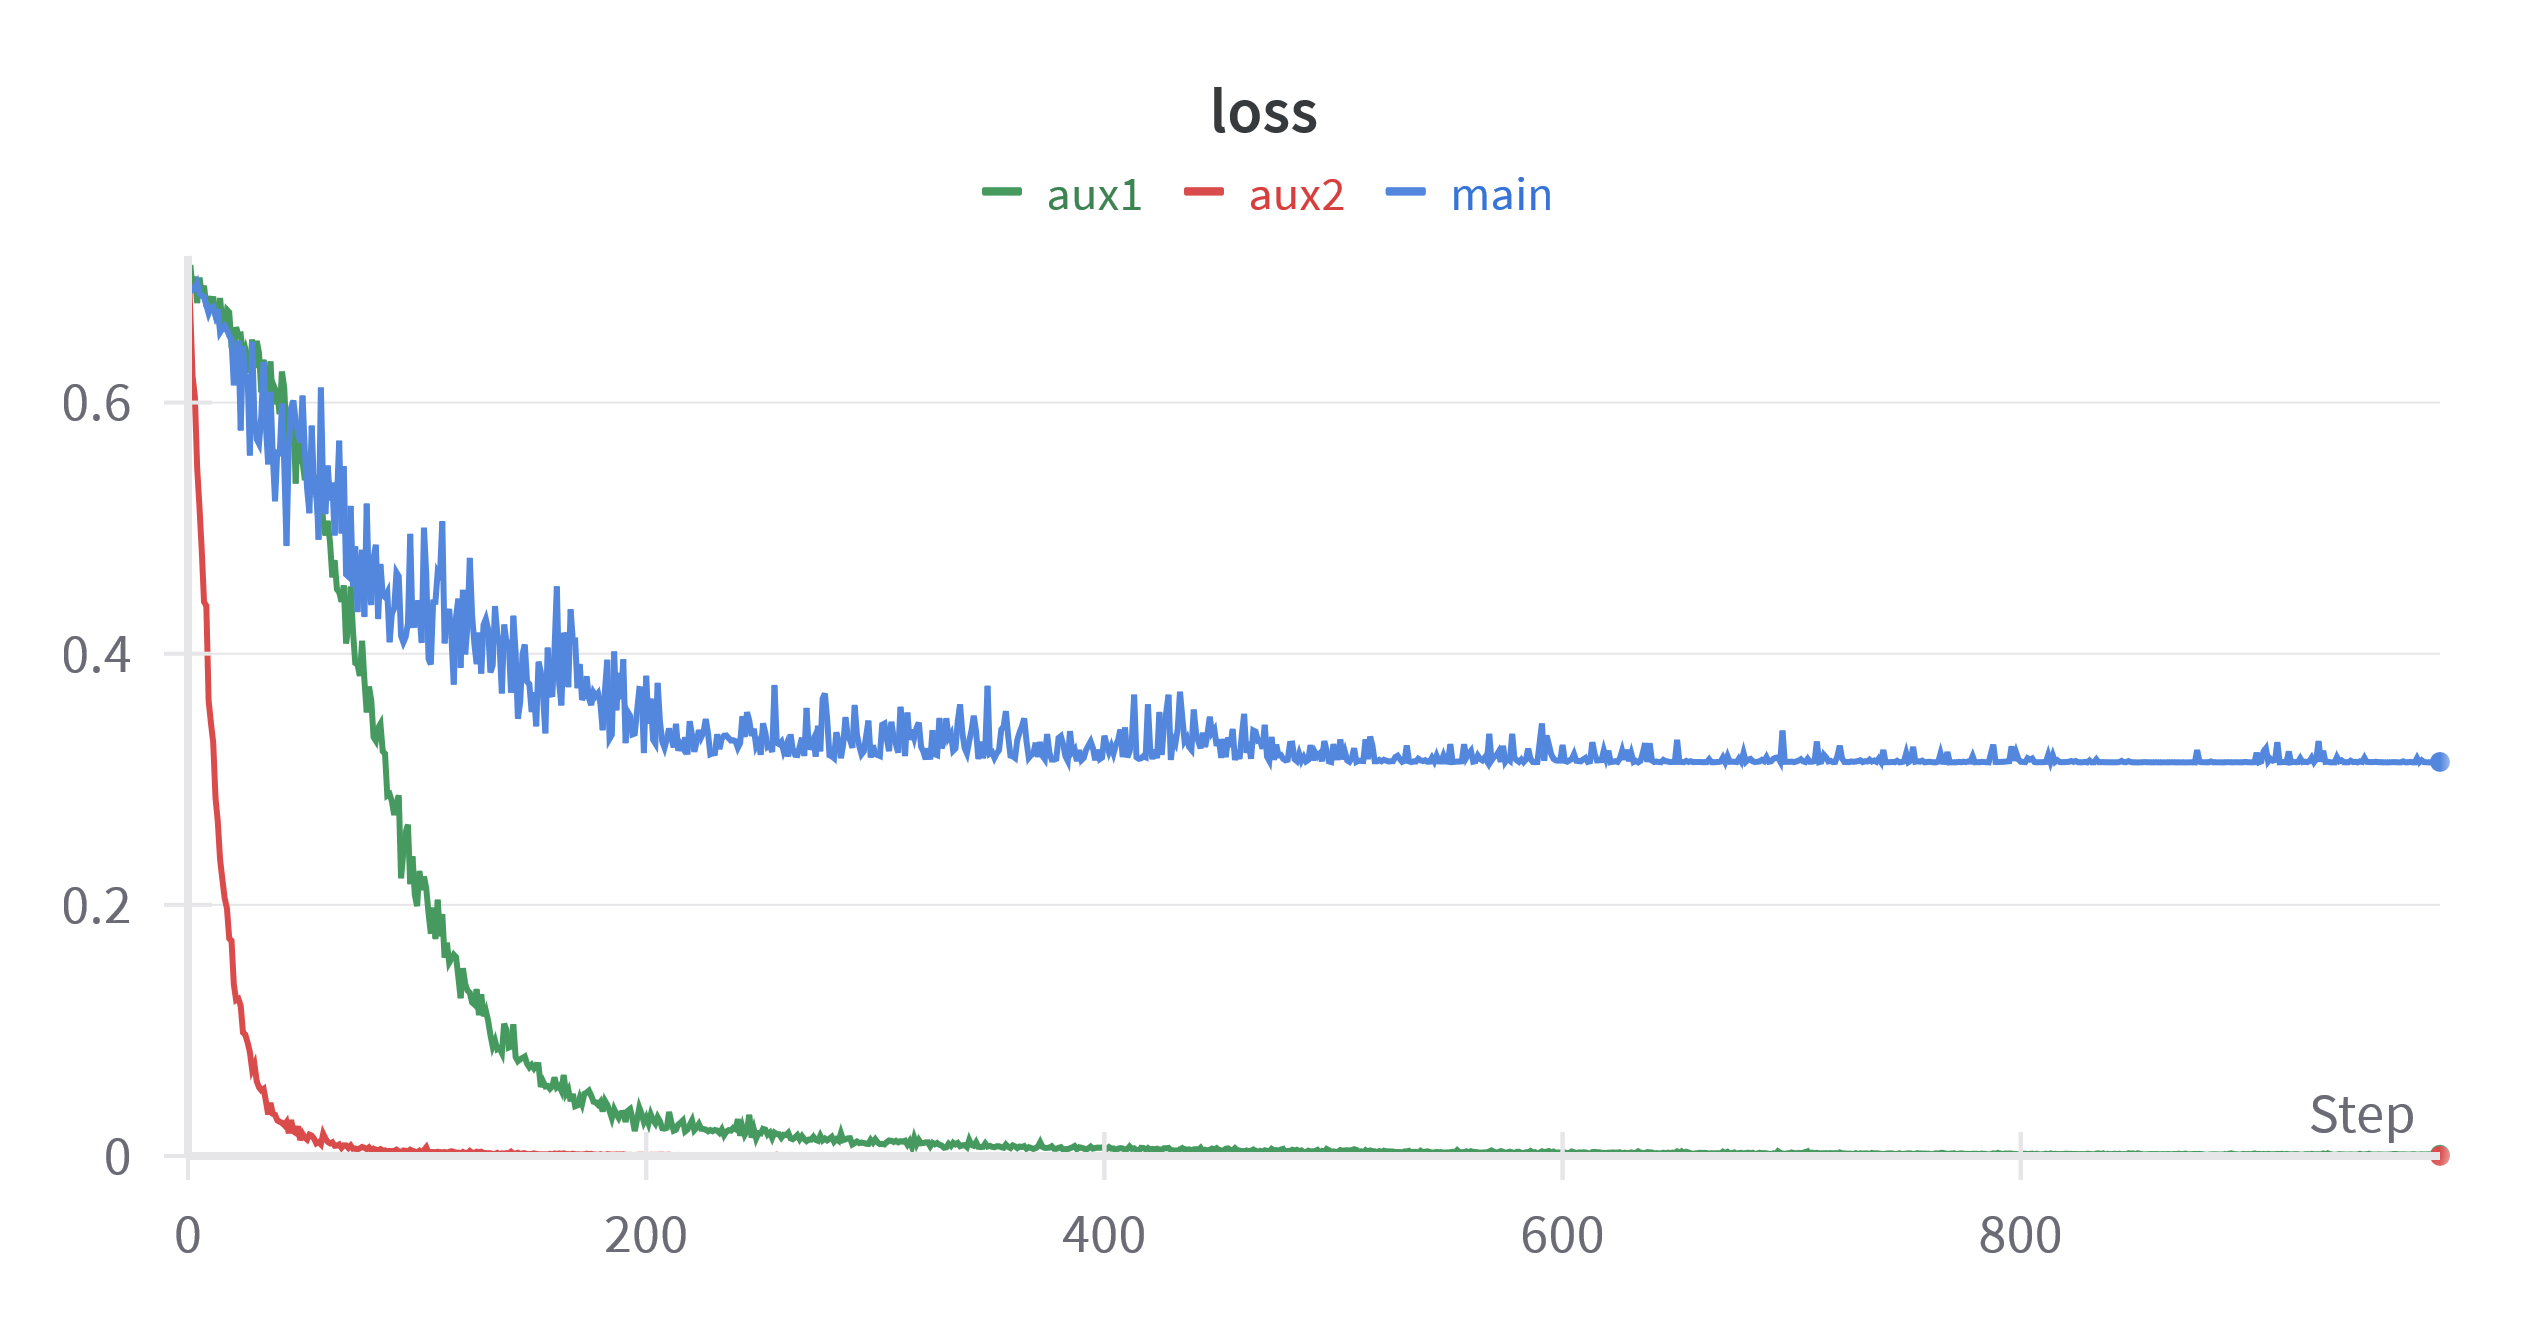
\includegraphics[width=1\linewidth]{figures/Figure19.png}
    \caption{Loss graph}
    \label{fig:fig18}
\end{figure}
Even with all these experiments and improvements, the best accuracy I managed to obtain was 0.5409. Towards the end of the process of training the classification model, I decided to use already trained weights from the Torchvision library. These weights had been trained on images from ImageNet. I also resized the images again and made them 512x512 in order to also fit the detection model. Figure \ref{fig:fig19} shows the loss graph after training the model for 5 epochs, while figure \ref{fig:fig20} shows the confusion matrix at the end of those epochs.\\
\begin{figure}[ht!]
    \centering
    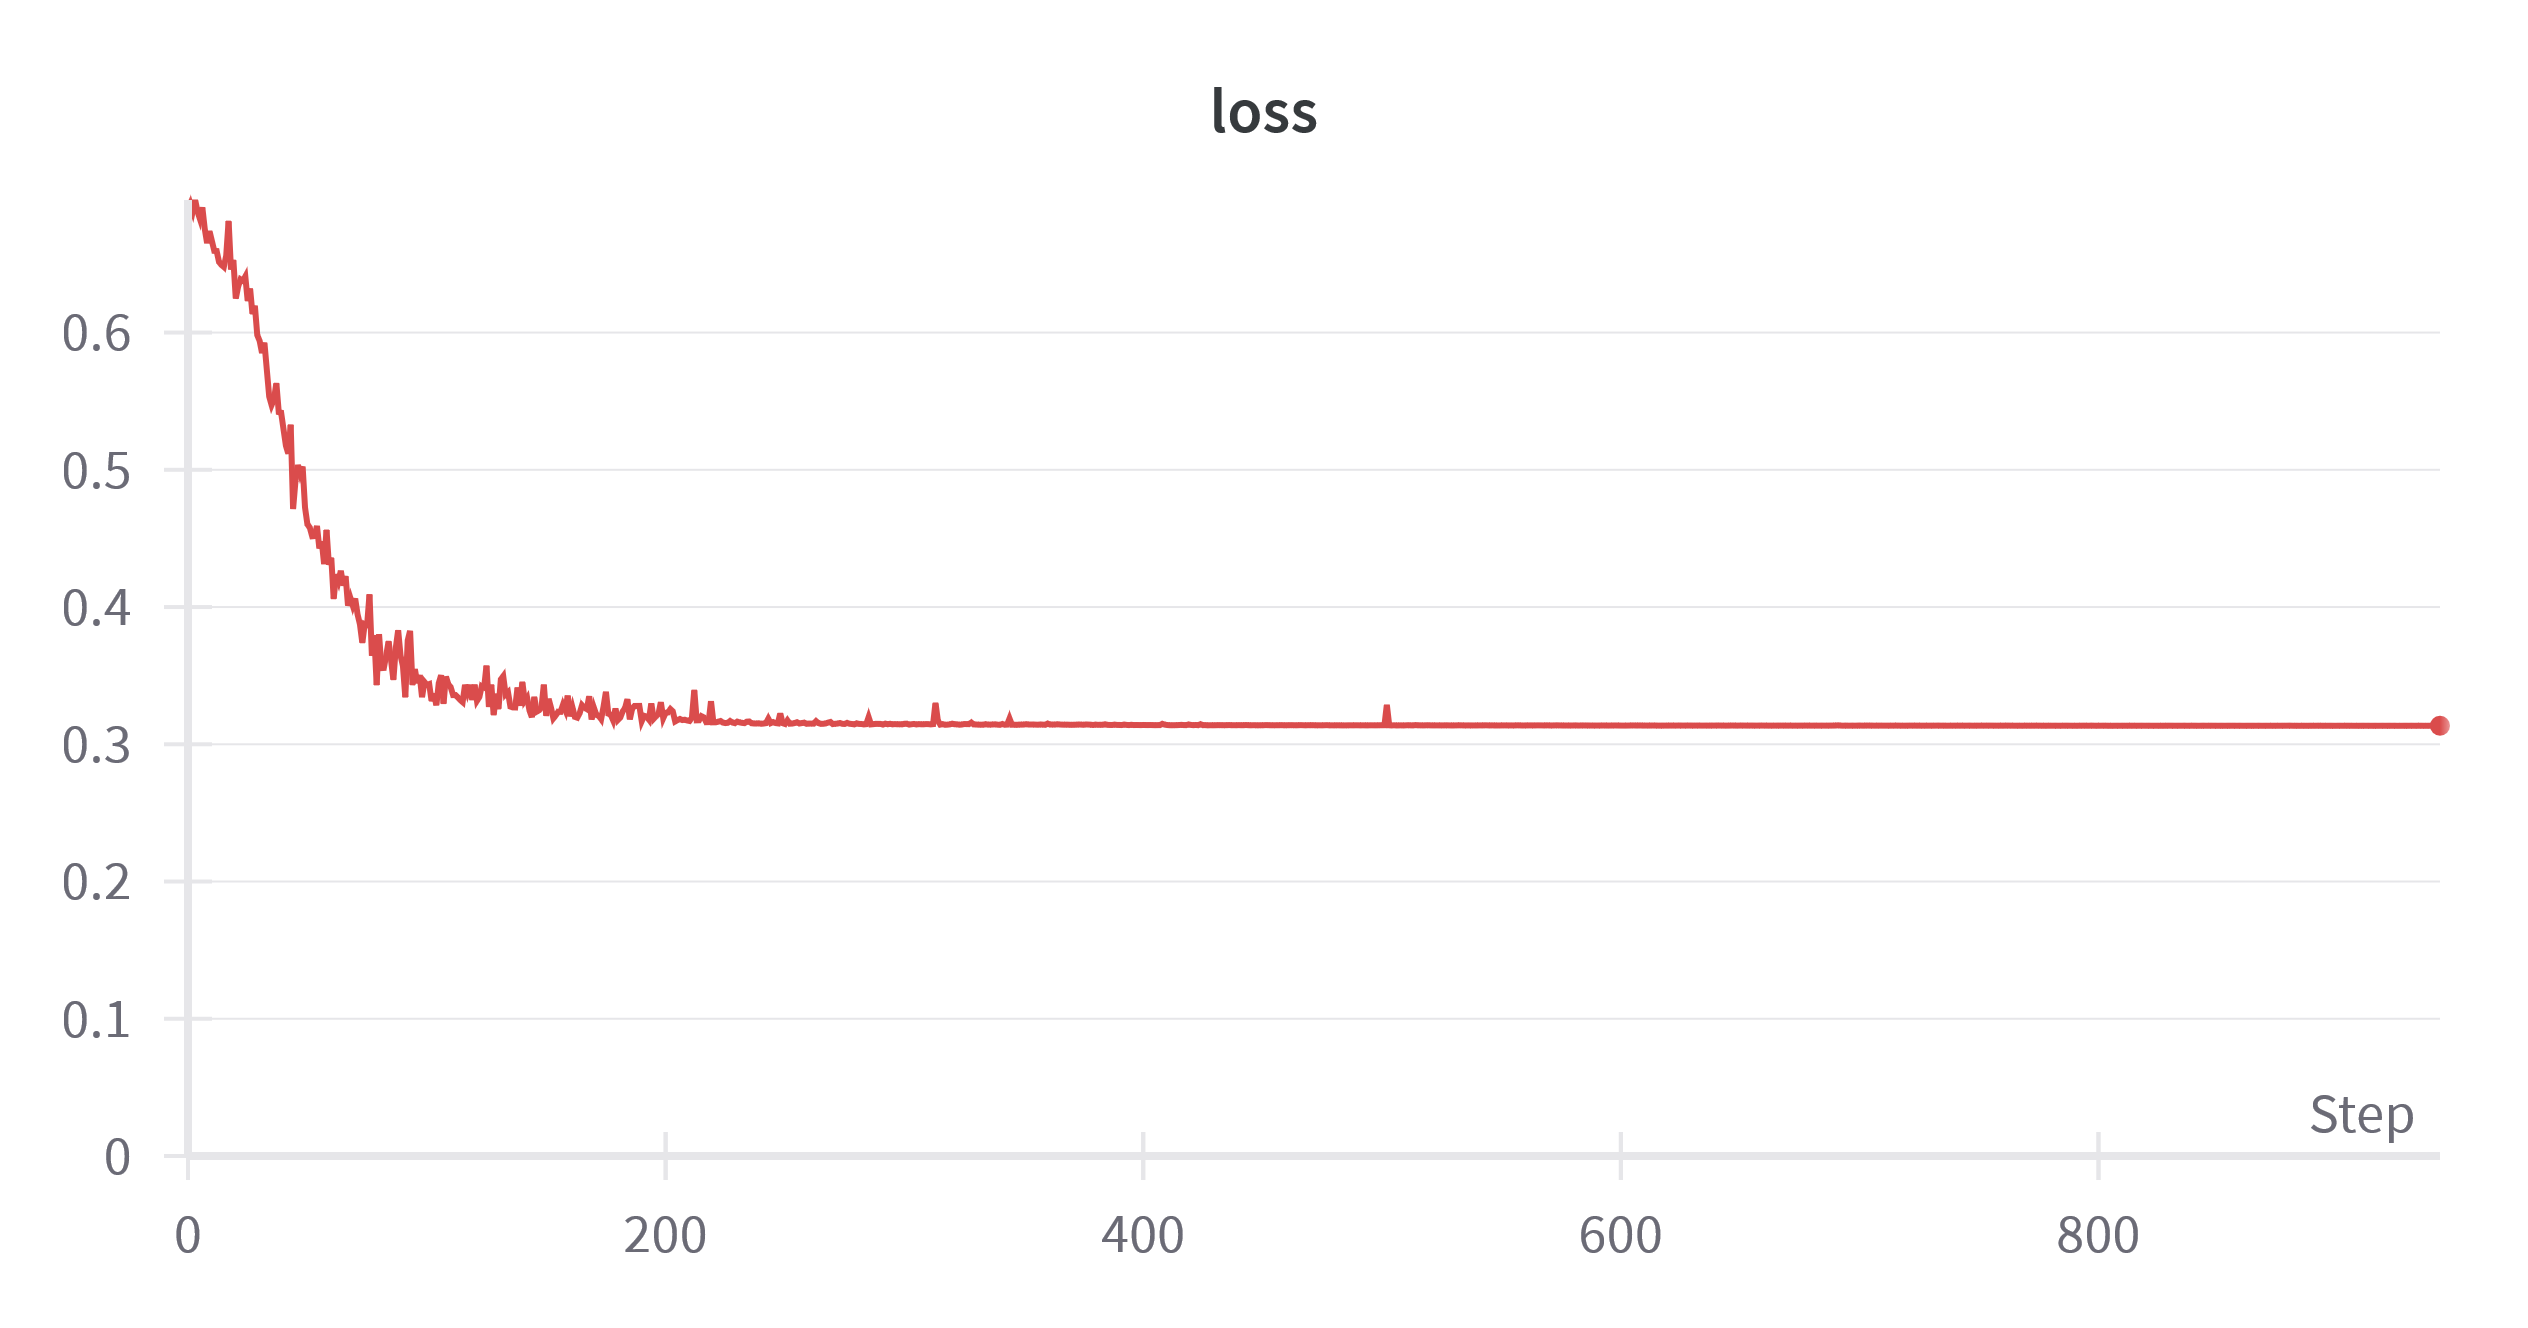
\includegraphics[width=1\linewidth]{figures/Figure20.png}
    \caption{Loss graph}
    \label{fig:fig19}
\end{figure}
\begin{figure}[ht!]
    \centering
    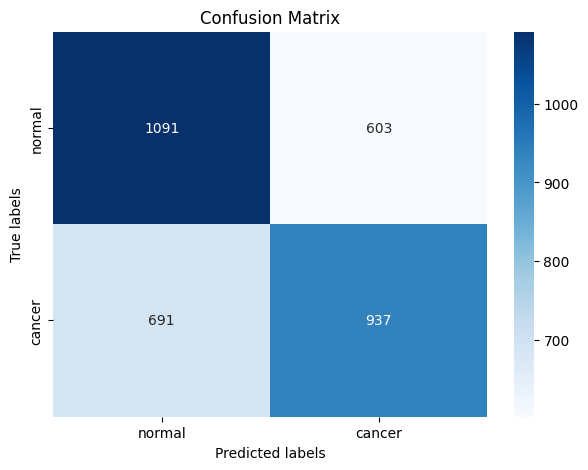
\includegraphics[width=0.5\linewidth]{figures/Figure21.png}
    \caption{After epoch 5}
    \label{fig:fig20}
\end{figure}
I also experimented with different batch sizes for the model. Therefore, I also trained the model with the same configuration as the previous run, except I modified the size of the batches from 64 to 128. Below is the comparison in loss between these two experiments. This second model I also trained for 5 epochs; however, the difference in steps in the graph comes from increasing the number of inputs in each batch, which means fewer batches over the dataset and overall fewer steps.\\
\begin{figure}[ht!]
    \centering
    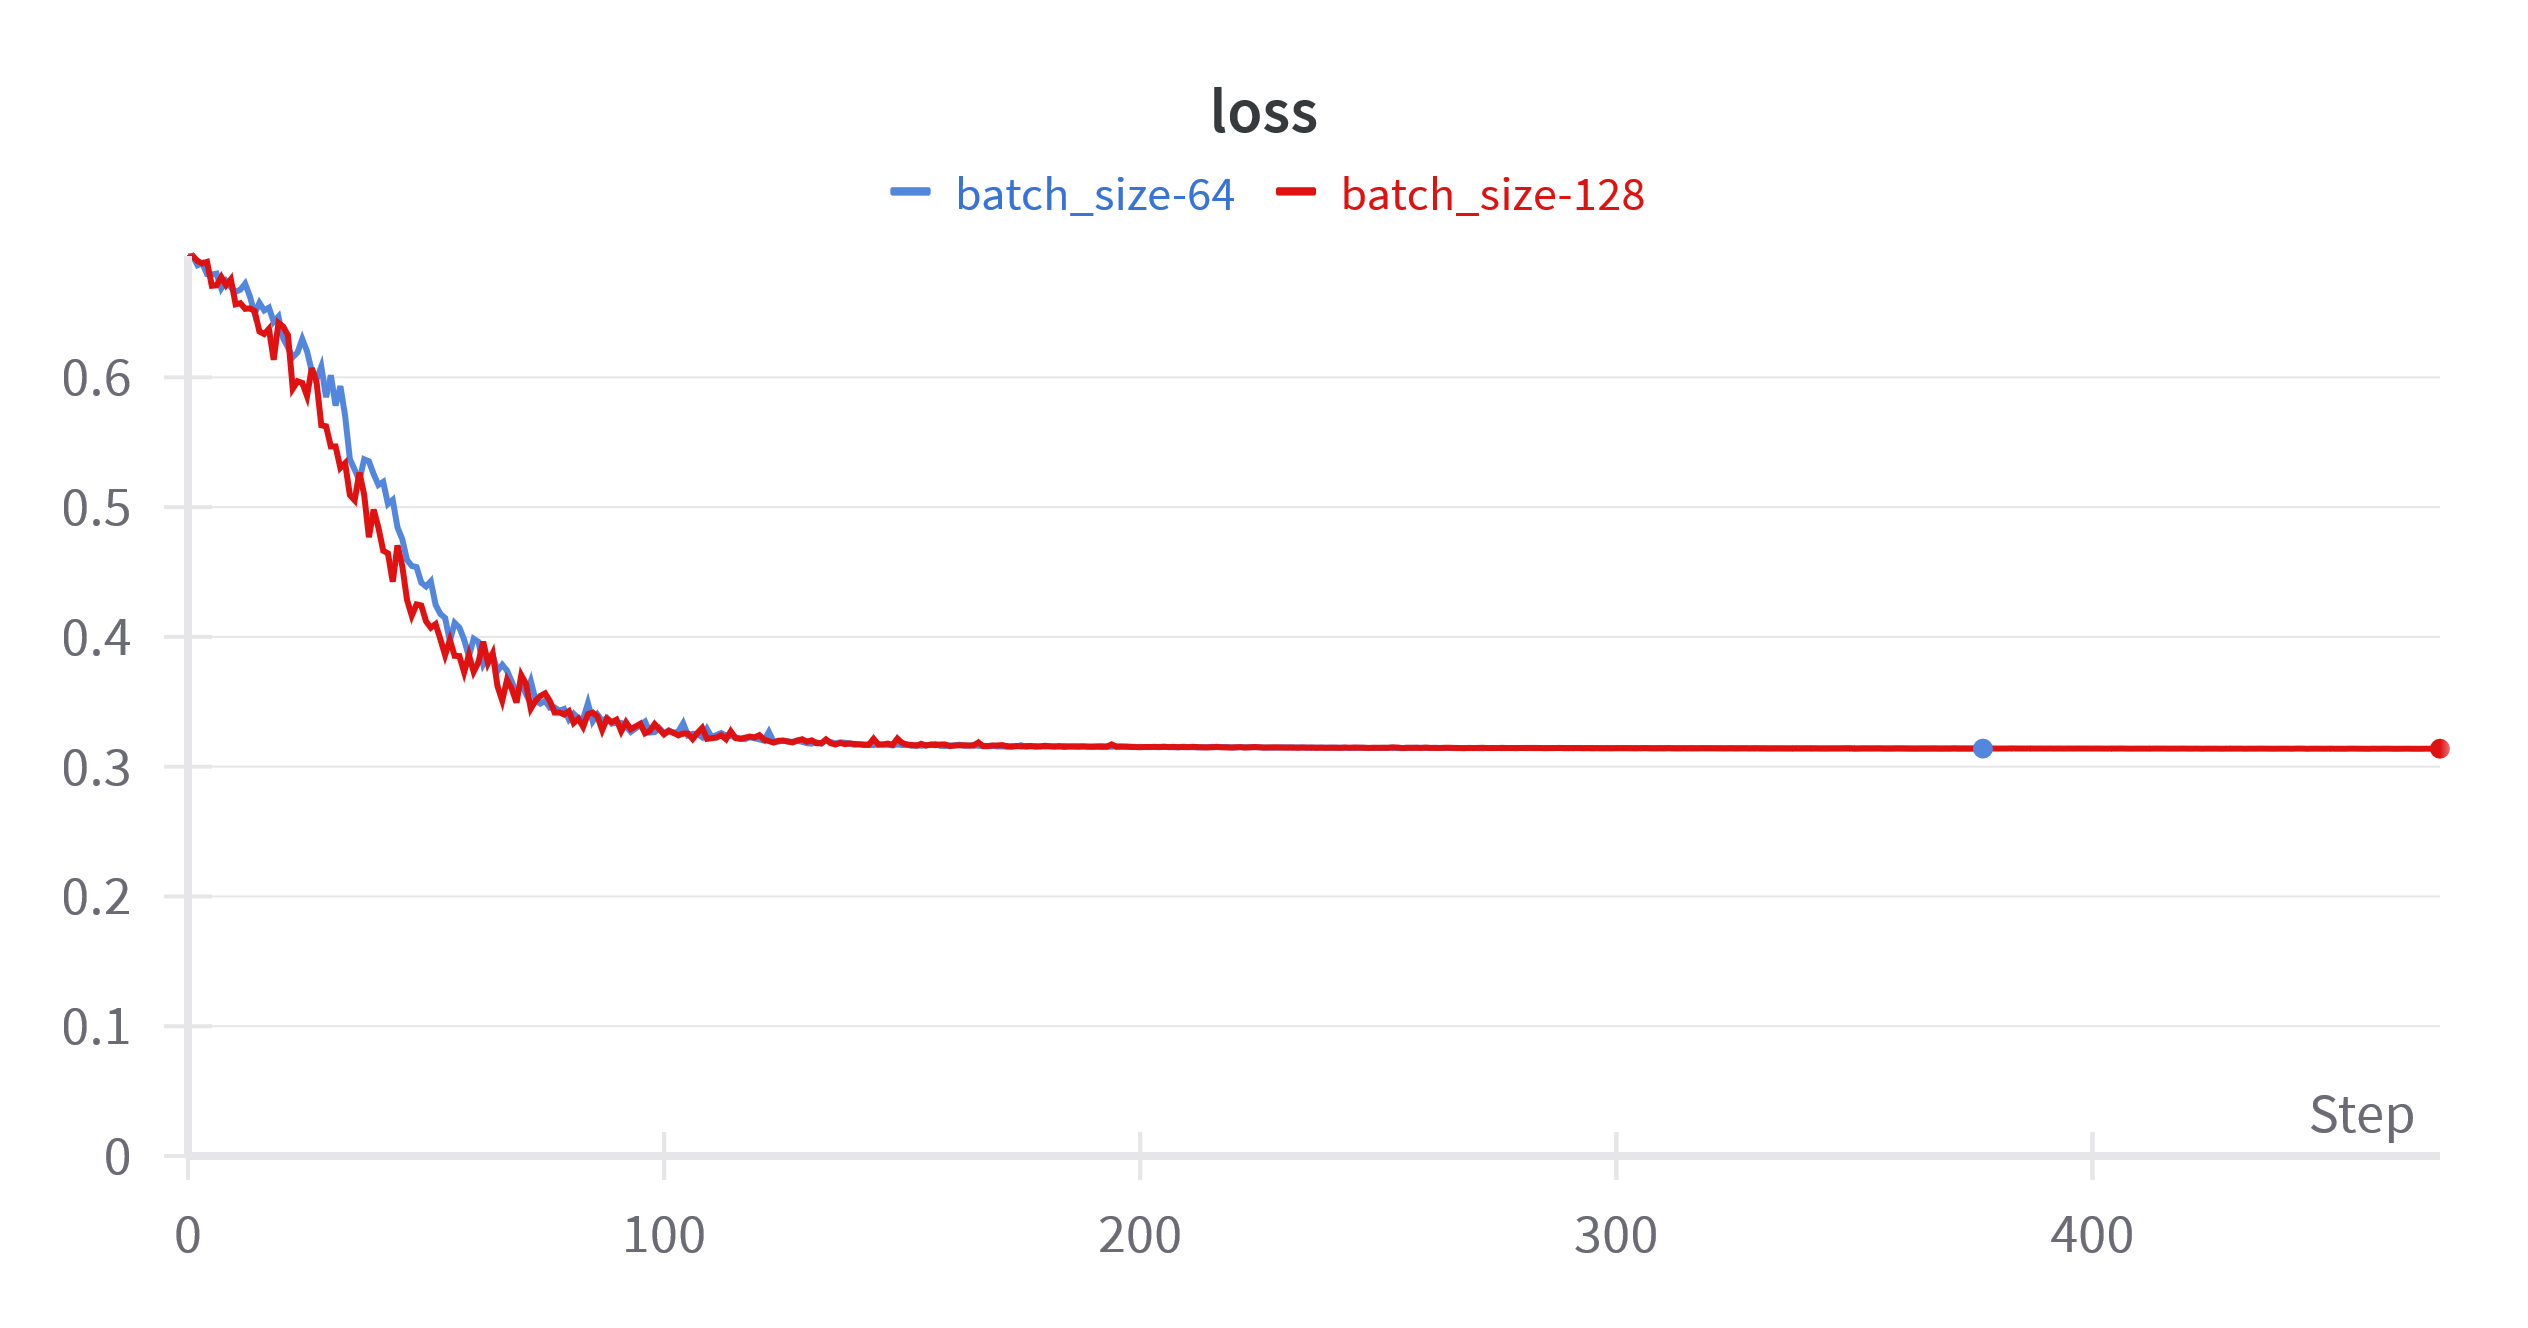
\includegraphics[width=1\linewidth]{figures/Figure22.png}
    \caption{Loss graph}
    \label{fig:fig21}
\end{figure}
The final configuration that I came to included: batches of size 128, pre-trained weights trained with images from ImageNet, a learning rate of 0.0001, learning rate decay using the StepLR implementation with a step size of 5 and gamma of 0.1, an image size of 512, and 22 inputs of each image representing different slices from the 3D scans. The loss obtained using a learning rate of Step instead of Exponential is shown in figure \ref{fig:fig22}.\\
\begin{figure}[ht!]
    \centering
    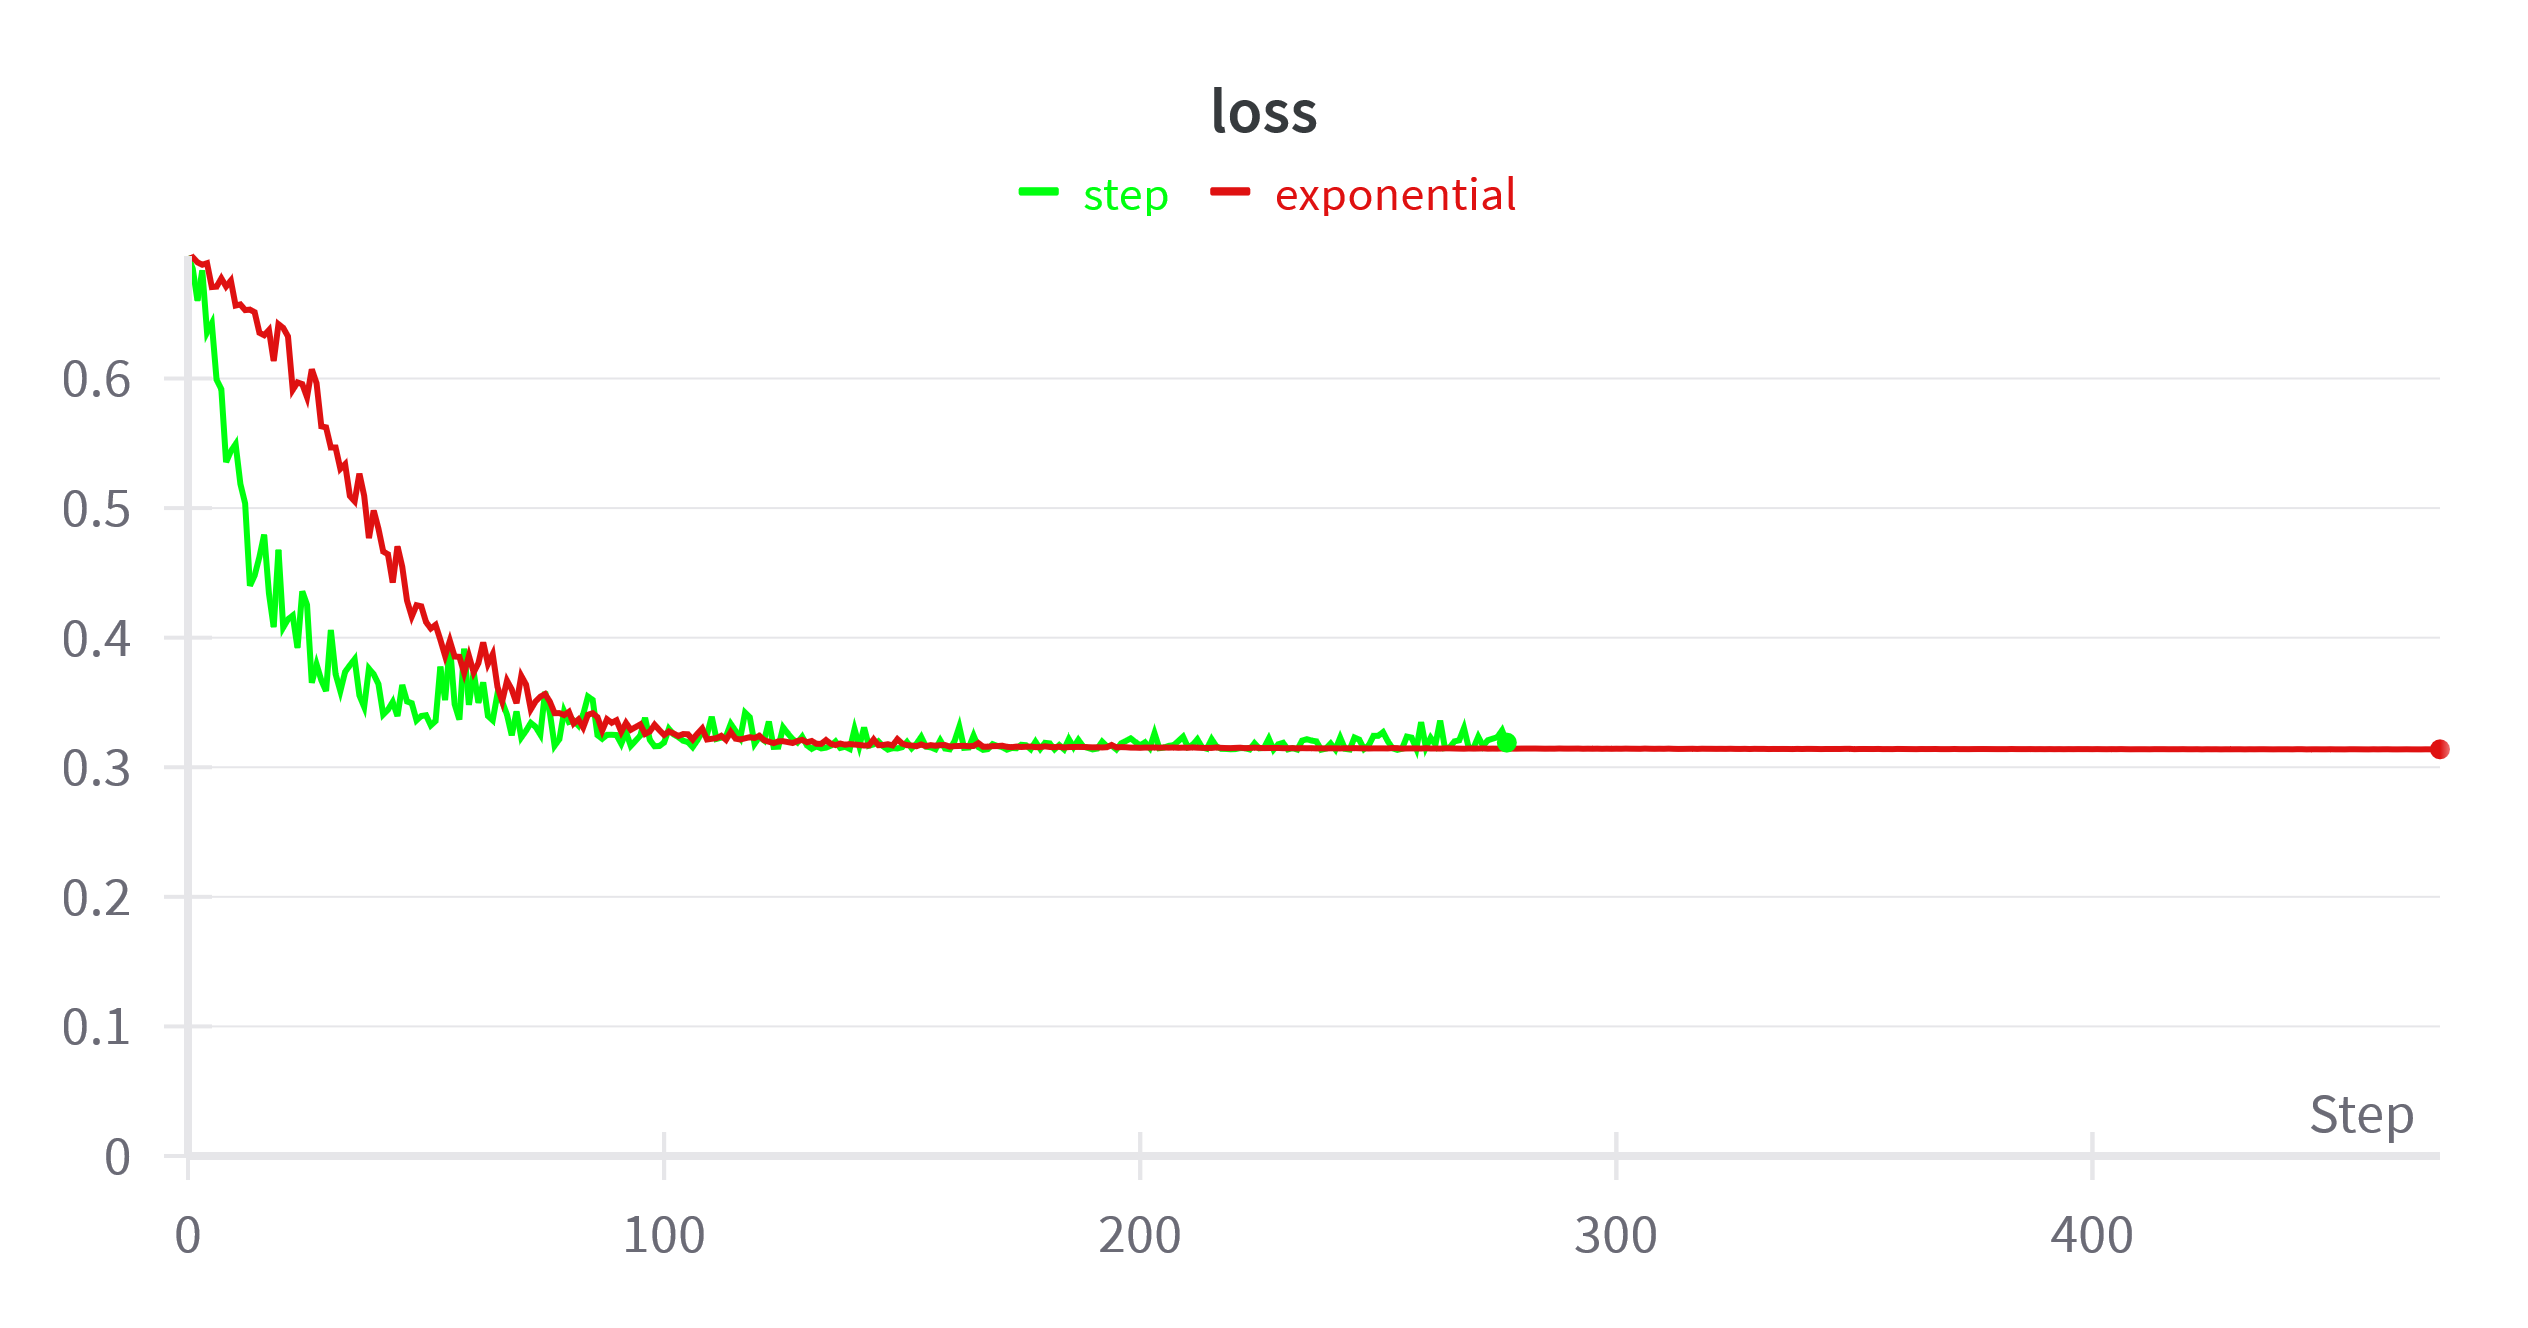
\includegraphics[width=1\linewidth]{figures/Figure24.png}
    \caption{Loss graph}
    \label{fig:fig22}
\end{figure}
\section{Detection experiments}